\documentclass{standalone}
\usepackage{tikz}
\usetikzlibrary{shapes.geometric, shapes, arrows,calc,positioning}

\begin{document}

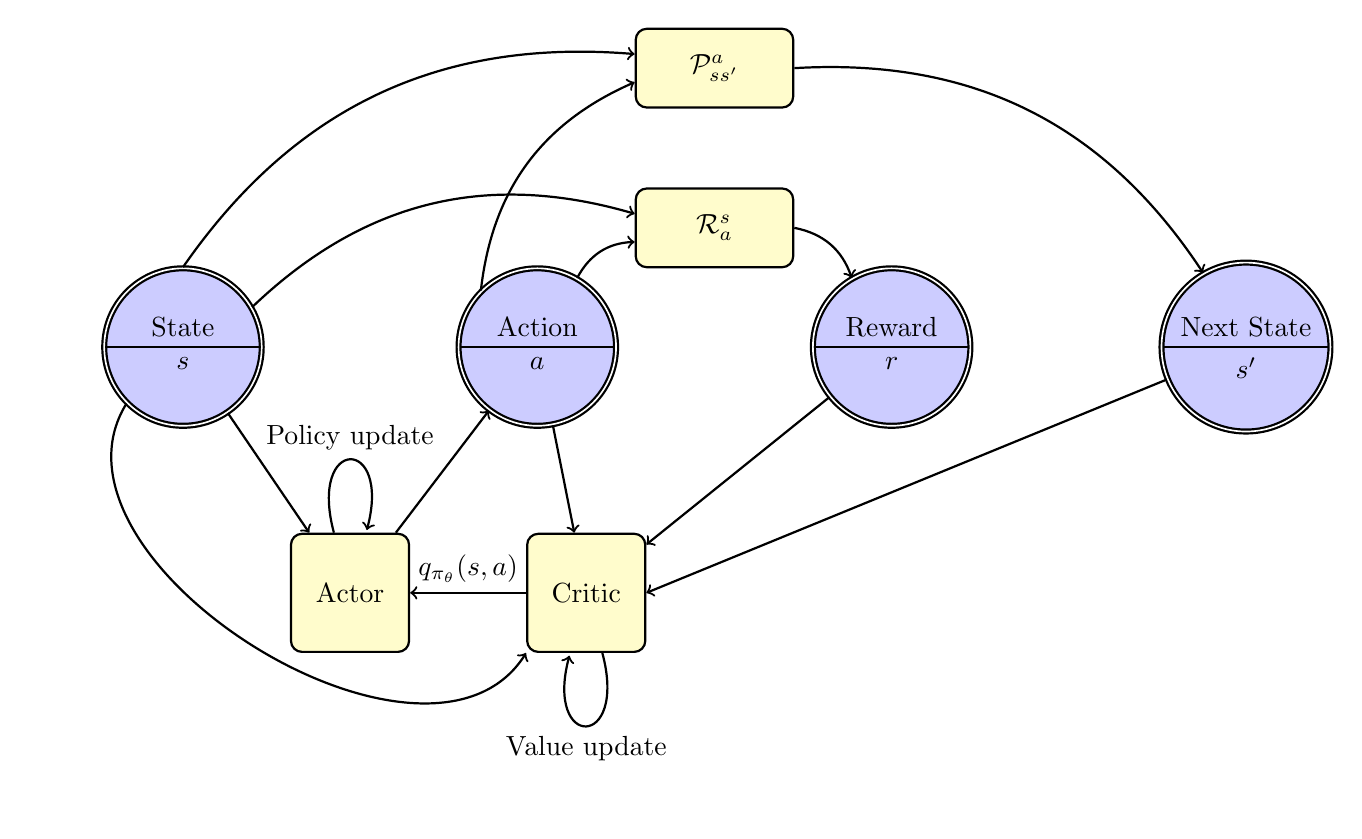
\begin{tikzpicture}[
		node distance=3cm,
		thick,
		signal/.style={draw,thick,circle,fill=blue!20},
		process/.style={draw,thick,minimum width=2cm,minimum height=1cm,rounded corners,fill=yellow!20,inner sep=.3cm},
		multimodal/.style={circle split,draw,double,fill=blue!20},
		state/.style={multimodal, minimum size=2cm},
		action/.style={multimodal, minimum size=2cm},
		reward/.style={multimodal, minimum size=2cm},
		actor/.style={process, minimum size=1.5cm, text centered},
		critic/.style={process, minimum size=1.5cm, text centered},
	]

	% Actor-Critic components
	\node[actor] (actor) {Actor};
	\node[critic, right of=actor] (critic) {Critic};

	% Agent's environment interaction
	\node[state, above left of=actor, yshift=1cm] (state) {State \nodepart{lower} $s$};
	\node[action, right of=state, xshift=1.5cm] (action) {Action \nodepart{lower} $a$};
	\node[reward, right of=action, xshift=1.5cm] (reward) {Reward \nodepart{lower} $r$};
	\coordinate (A) at ($(action)!0.5!(reward)$);
	\node[process, above = 1 of A] (rsa) {$\mathcal{R}_a^s$};
	\node[process, above = 1 of rsa] (transition) {$\mathcal{P}_{ss'}^{a}$};

	\node[state, right of=reward, xshift=1.5cm] (next_state) {Next State\nodepart{lower} $s'$};

	% Arrows connecting the components
	%\path[->] (state) edge [bend left=30] node[above, sloped] {Policy} (action);
	%\path[->] (action) edge node[above, sloped] {$\mathcal{R}_a^s$} (reward);
	\path[->] (state.90) edge [bend left=30] (transition.170);
	\path[->] (action.135) edge [bend left=30] (transition.190);
	\path[->] (state.30) edge [bend left] (rsa.170);
	\path[->] (action.60) edge [bend left=30] (rsa.190);
	\path[->] (rsa.0) edge [bend left] (reward.120);
	\path[->] (transition.0) edge [bend left] (next_state.120);
	%\path[->] (action) edge [bend left=30] node[above, sloped] {$\mathcal{P}_{ss'}^{a}$} (next_state);
	%\path[->] (next_state.90) edge [bend right=40] node[above, sloped] {Update} (state.45);

	% Arrows connecting actor and critic
	\path[->] (state) edge (actor);
	\path[->] (state.225) edge [bend right=90] (critic.225);
	\path[->] (actor) edge (action);
	\path[->] (reward) edge (critic);
	\path[->] (action) edge (critic);
	\path[->] (next_state) edge (critic.0);
	\path[->] (critic) edge node[above] {$q_{\pi_{\theta}}(s,a)$} (actor);

	% Data flow within the components
	\path[->] (actor) edge [loop above] node[above] {Policy update} (actor);
	\path[->] (critic) edge [loop below] node[below] {Value update} (critic);

\end{tikzpicture}

\end{document}
